\documentclass{scrreprt}
\usepackage[ngerman]{babel}
\usepackage[utf8]{inputenc}
\usepackage[T1]{fontenc}
\usepackage{amsthm}
\usepackage{lmodern}
\usepackage{graphicx}
\usepackage{amsthm}
\usepackage{listings}


\newtheorem{Definition}{Definition}

%Macros:

%Text-Overline:
\newcommand{\textoverline}[1]{$\overline{\mbox{#1}}$}
%PANDA: 
\newcommand{\pnd}{\textoverline{P}ANDA}

%code
\newcommand{\code}[1]{\nobreak{\textbf{#1}}}
 
\title{Seminararbeit}
\author{Felix Kibellus}
 
\begin{document}
\maketitle
\tableofcontents
 
\chapter{Einleitung}
Die Hadronenphysik beschäftigt sich mit der inneren Struktur von Atomkernen. Die Beobachtung komplexer Zerfallsketten liefern physikalisch interessante Erkenntnisse und stellen eine Möglichkeit dar, um Rückschlüsse auf die innere Teilchenstruktur ziehen zu können. Da die meisten solcher Ereignisse nicht stabil vorkommen werden Teilchenbeschleuniger eingesetzt, welche durch hohe Energiezuführung das Entstehen von physikalisch interessanten Teilchen herbeiführen. Bei der Konstruktion solcher Großgeräte handelt es sich um ein breites Aufgabenfeld. Zur physikalischen Analyse des Experiments sind die Kenngrößen Impuls, Energie, Art und Spur des Teilchens von Interesse. Zu deren Erfassung ist ein komplexes Detektorsystem nötig. Dieses besteht unter anderem aus Detektoren zur Rekonstruktion von Teilchenflugbahnen. Ein solcher spurgebender Detektor ist in der Lage einen sogenannten Hit zu melden, wenn ein Teilchen eine bestimmte Position passiert hat. Zur Auswertung dieser Detektoren werden Spurfindungs-Algorithmen eingesetzt. Diese versuchen aus den gemessenen Hits die Teilchenflugbahn zu rekonstruieren. Da es unmöglich ist einen perfekten Trackfinding-Algorithmus zu entwickeln, sind die rekonstruierten Tracks fehlerbehaftet. Somit ist es möglich, dass ein solcher Algorithmus Hits zu einem Track hinzufügt, welche in Wirklichkeit zu einem anderen physikalischen Track gehören. Um solche Tracks im Nachhinein von falschen Hits bestmöglich zu reinigen ist im Rahmen dieser Arbeit ein sogenannter Track-Cleaner entstanden. Zur Realisierung wurde für jeden Hit der Abstand zum approximierten Track bestimmt und ermittelt ob dieser Abstand einen parametrisierbaren Grenzwert $\mu$ überschreitet. Der Track-Cleaner ist im Rahmen des \pnd{}-Experiments entwickelt und getestet worden, kann jedoch prinzipiell für alle ähnlichen Experimente eingesetzt werden, da er unabhängig vom verwendeten Trackfinder und Detektorsystem funktioniert. Das \pnd{}-Experiment ist ein Teil der Teilchenbeschleunigeranlage FAIR, welche zur Zeit in Darmstadt entsteht. Im folgenden Kapitel wird zunächst auf FAIR eingegangen und das Detektorsystem \pnd{} erklärt. Anschließend wird das verwendete Framework Root erörtert und schließlich die Entwicklung des Trackfinders dokumentiert. Im letzten Kapitel wird erklärt, wie mittels einer Parameterstudie der optimale Grenzwert $\mu$ gefunden wurde.
\chapter{Die Beschleunigeranlage FAIR unter besonderer Betrachtung des \pnd{}-Detektors}

Da der Track-Cleaner in Zusammenhang mit dem \pnd{}-Experiment entwickelt wurde, soll nun auf das zugrunde liegende physikalische Experiment eingegangen werden. Dazu wird zunächst die Beschleunigeranlage FAIR erklärt, um dann im weiteren Verlauf des Kapitels den \pnd{}-Detektor zu erläutern. Da der \pnd{}-Detektor aus mehreren Subdetektoren besteht, wird im Folgenden die Funktionsweise des Straw Tube Trackers (STT) thematisiert. In diesem Zusammenhang wird auf die Problematik des Trackfindings eingegangen, um somit die Entwicklung eines Track-Cleaners zu motivieren.

\section{FAIR - Facility for Antiproton and Ion Research}
\begin{figure}
  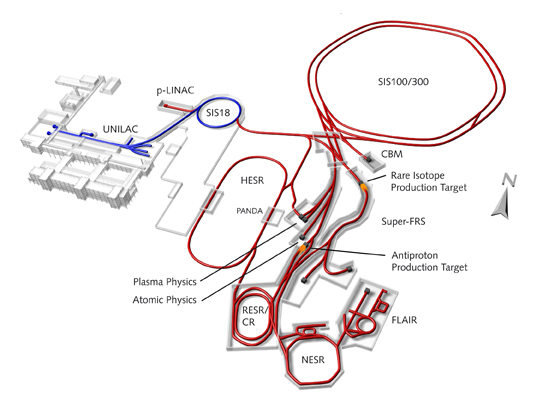
\includegraphics[width=0.7\textwidth]{Bilder/Fair}
	\label{fig:FAIR}
	\caption{Schematische Darstellung der Beschleunigeranlage FAIR}
\end{figure}

Eine schematische Darstellung von FAIR findet sich in Abbildung \ref{fig:FAIR}. Die bereits bestehenden Komponenten der Gesellschaft für Schwerionenforschung sind in blau dargestellt und werden in FAIR integriert. Diese sind in der Abbildung mit SIS18 bezeichnet und werden in Zukunft als Vorbeschleuniger für Protonen benutzt. Diese werden danach in den Doppelring (SIS100) eingespeist und auf bis zu 29GeV beschleunigt. GeV steht für die kinetische Energie in Giga-Elektronvolt. Die Beschleunigung eines Protons auf 29GeV entspricht einer Geschwindigkeit von $2.9\cdot10^8\frac{m}{s}$ bzw. dem 0.9995-fachen der Lichtgeschwindigkeit. Da in FAIR mehrere Experimente zusammengefasst werden sollen, schließen sich danach mehrere Möglichkeiten der Strahlführung an, um den Teilchenstrahl auf die verschiedenen Experimente zu verteilen. Für das \pnd{}-Experiment wird der Strahl zunächst auf ein Wolfram-Target geschossen, um die für \pnd{} benötigten Antiprotonen zu erzeugen. Diese werden dann im Collector Ring (CR) gesammelt, gekühlt und in den High-Energy Storage Ring (HESR) eingespeist. Dort werden die Antiprotonen zunächst auf 14.5 GeV beschleunigt und dann in das am HESR platzierte \pnd{}-Experiment eingeführt. Darauf wird nun im Folgenden genauer eingegangen. \cite[S. 5]{MasterJette}



\section{\pnd{} - Antiproton ANnhilation at DArmstadt}
\label{sec:Panda}
Um die Funktionsweise des Trackfindings zu verstehen, wird nun zunächst der \pnd{}-Detektor erklärt. Dazu wird zuerst auf die physikalische Bedeutung von \pnd{} eingegangen und später der Aufbau des Detektors erläutert.

\subsection{Physikalische Bedeutung von \pnd{}}
\pnd{} beschäftigt sich mit der starken Kraft und den damit zusammenhängenden Wechselwirkungen. Die starke Kraft ist dafür verantwortlich, dass die Nukleonen eines Atomkerns zusammengehalten werden. Durch Experimente mit hochenergetischen Antiprotonenstrahlen soll in \pnd{} die starke Kraft untersucht werden. Dabei werden Antiproton-Proton-Annihilationen und die Reaktionen von Antiprotonen mit schweren Kernen betrachtet. Annihilation beschreibt den Prozess der Paarvernichtung eines Fundamentalteilchens, welches mit seinem korrespondierenden Antiteilchen zusammenstößt. 
\cite[S. 5]{MasterJette} 

\pnd{} wurde so konstruiert, dass verschiedene Experimente mit dem selben Detektorsystem durchgeführt werden können. Diese Experimente lassen sich wie folgt klassifizieren \cite{PANDA_physics_overview}:

\label{panda_experimentklassen}
\begin{description}
	\item[Hadronenspektroskopie] Dieses Aufgabenfeld beschäftigt sich mit der Suche nach exotischen Anregungszuständen von Hadronen. Damit soll die starke Wechselwirkung genauer untersucht werden.
	\item[Nukleonenstruktur] Hier soll der innere Aufbau von Nukleonen genauer erforscht werden, um Rückschlüsse auf Struktur und Bestandteile von Atomkernen ziehen zu können.
	\item[Hadronen in Materie] Um den Ursprung der Hadronenmasse zu verstehen, sollen Hadronen in einem Nuklearen Medium untersucht werden.
	\item[Hyperkerne] Wird bei einem Nukleon ein up- oder ein down-Quark durch ein Strange-Quark ersetzt entstehen Hyperkerne. Durch die Einführung der Strangeness entsteht ein weiterer Freiheitsgrad und somit eine weitere Achse im Nuklear-Diagramm. Diese neuartigen Elemente sollen genauer untersucht werden.
\end{description}

\subsection{Aufbau des Detektors}
\begin{figure}
  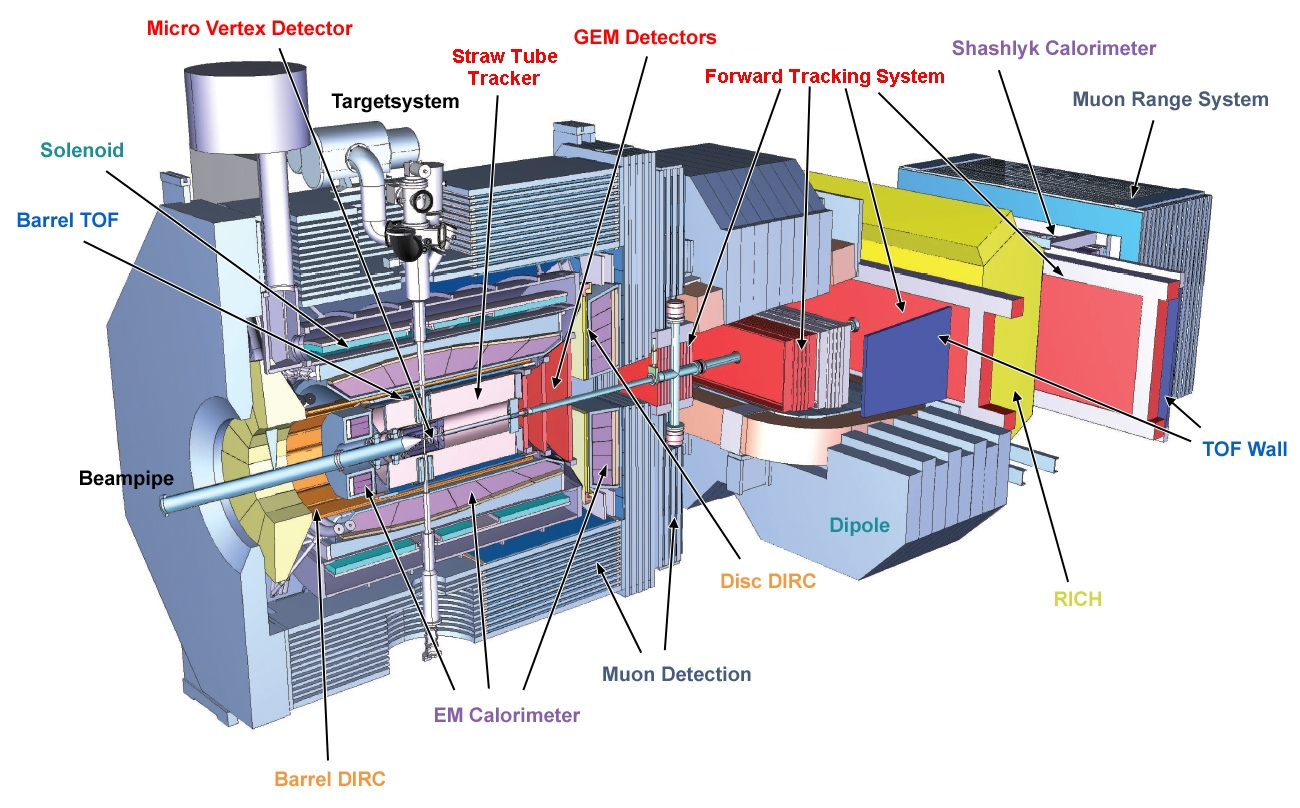
\includegraphics[width=0.9\textwidth]{Bilder/panda_full_detektor}
	\label{fig:panda_full}
	\caption{Schematische Darstellung des gesamten \pnd{}-Detektors}
\end{figure}
Bei dem \pnd{}-Detektor handelt es sich um ein komplexes Detektorsystem, welches aus vielen verschiedenen Subdetektoren zusammengesetzt ist. Eine schematische Darstellung des gesamten \pnd{}-Detektors findet sich in Abbildung \ref{fig:panda_full}. Über das Strahlrohr gelangt der Antiprotonenstrahl zum zentral platzierten Targetsystem. Das Targetsystem ist austauschbar, sodass es an die in Abschnitt \ref{panda_experimentklassen} erwähnten Experimenttypen angepasst werden kann. Das Targetmaterial lässt sich über das Targetsystem zum Stoßpunkt befördern, wo es dann mit dem Antiprotonenstrahl kollidiert. Dabei entsteht eine große Anzahl an Sekundärteilchen, welche sich vom Stoßpunkt aus in verschiedene Richtungen bewegen. Um aus dem Experiment physikalisch wertvolle Ergebnisse folgern zu können, müssen die entstandenen Teilchen möglichst genau rekonstruiert werden. Dazu befindet sich eine Vielzahl unterschiedlicher Detektoren um den Stoßpunkt herum. Diese lassen sich aufgrund ihrer Aufgabe kategorisieren. Der Micro-Vertex-Detektor (MVD), der Straw Tube Tracker/Central Tracker (STT), der Gas Electron Multiplier Detector (GEM), und das Forward Tracking System (FTS) sind spurgebende Detektoren, welche versuchen die Teilchenflugbahn zu rekonstruieren. Darüber hinaus gibt es die Detektoren Detection of Internally Reflected Cherenkov Light (DIRC), Time of Flight System (TOF) und Aerogel Ring Imaging Cherenkov Counter (RICH), welche zur Teilchenidentifikation dienen. Zur Impulsbestimmung befindet sich sowohl im vorderen, als auch im hinteren Teil des \pnd{}-Detektors ein Magnetspektrometer . Das Target-Spektrometer mit einem 2T Solenoid Magnetfeld befindet sich beim Stoßpunkt. Beim Forward-Spektrometer handelt es sich um ein 2Tm Dipol-Magnetfeld, welches sich im hinteren des Detektors befindet. Somit lässt sich der Detektor als Ganzes in zwei Teile aufteilen. Mit dem Target-Spektrometer werden die Teilchen erfasst, deren Flugbahn einen vergleichsweise hohen Polarwinkel aufweisen. Das Forward-Spektrometer erfasst die Teilchen, welche sich im Wesentlichen in Richtung des Antiprotonenstrahls bewegen. Die Funktionsweise der Magnetspektrometern macht sich die Eigenschaften der Lorentzkraft zu Nutze. Ein geladenes Teilchen erfährt beim Durchqueren eines Magnetfeldes $B$ die Kraft $\vec{F_L}=q(\vec{v} \times \vec{B})$, wobei $\vec{v}$ die Bewegungsrichtung, $\vec{B}$ die magnetische Flussdichte und $q$ die Ladung ist. Bei Kenntnis von Teilchenflugbahn und Magnetfeldstärke lassen sich also Rückschlüsse auf die Ladung des Teilchens $q$ ziehen. Die Magneten selber erzeugen dabei keine Messwerte, sondern verursachen nur das zur Ablenkung des Teilchens benötigte Magnetfeld. \cite{PANDA_detektor} \cite[S. 7-10]{MasterJette}
Aufgrund der ablenkenden Wirkung des Magnetfeldes ergeben sich im Target-Spektrometer im Idealfall helixförmige Flugbahnen. Es kann jedoch zu Wechselwirkungen mit dem Detektormaterial kommen, was zum Energieverlust der Teilchen führt. In diesem Fall reduziert sich der Radius der Kreisbewegung mit fortschreitendem Energieverlust.
\cite[S. 11]{MasterJette}

\section{STT - Straw Tube Tracker}
\begin{figure}
  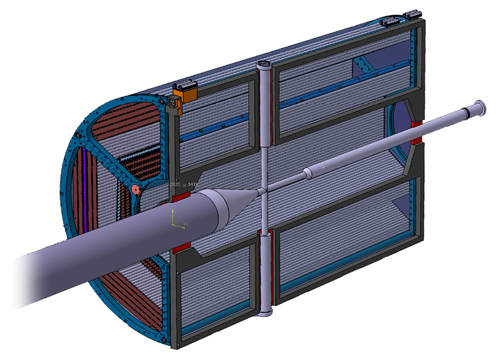
\includegraphics[width=0.9\textwidth]{Bilder/panda_stt}
	\label{fig:panda_stt}
	\caption{Schematische Darstellung des Straw Tube Trackers}
\end{figure}
Im Folgenden wird nun der Straw Tube Tracker genauer betrachtet. Beim STT handelt es sich, wie im vorangegangenen Abschnitt erläutert, um einen spurgebenden Detektor, dessen Aufgabe es ist Teilchenflugbahnen zu rekonstruieren. Wie in Abbildung \ref{fig:panda_stt} ersichtlich, umschließt der STT den Stoßpunkt. Die Aufgabe des STTs besteht darin, die spiralförmigen Flugbahnen von geladenen Teilchen mit möglichst hoher Auflösung zu messen. Dazu werden Driftröhrchen verwendet. Bei einem Driftröhrchen handelt es sich um einen mit Gas gefüllten Zylinder. Der Zylinder besitzt sowohl eine leitende Innenbeschichtung, als auch einen Draht in der Mitte an dem eine Hochspannung angelegt wird. Dadurch entsteht ein elektrisches Feld. Durchquert ein Teilchen die Straw-Tube führt dies dazu dass ein Gas-Molekül ein Elektron abspaltet, welches sich dann aufgrund des elektrischen Feldes zum Draht bewegt. Das positiv geladene Ion hingegen wandert zur Außenbeschichtung. Die Feldlinien verlaufen in der Nähe des Drahtes vergleichsweise dicht. Daher wird das Elektron schnell genug, um beim Zusammenstoß mit anderen Gasteilchen weitere Elektronen abzuspalten, welche sich ihrerseits wieder zum Draht bewegen. Dabei kommt es zum sogenannten Lawineneffekt, das Gas wird ionisiert. Dies führt dazu, dass es zu einer Verstärkung des ursprünglichen Signals kommt, welche von außen gemessen werden kann. Die Zeitspanne vom Eintreten eines Teilchens bis zu dem Zeitpunkt, wo das erste Elektron den Draht erreichen, wird als Drift-Zeit bezeichnet und kann verwendet werden, um den minimalen Abstand der Teilchenspur vom Draht zu berechnen. Dieser Abstand wird Isochronenradius genannt. Folglich lässt sich ein Zylindermantel (Isochron) mit dem Isochronenradius um den Draht herum konstruieren, welche alle möglichen minimalen Punkte enthält an dem das Teilchen den Draht passiert hat. Der STT liefert folglich nur eine zweidimensionale Auflösung, da nicht entschieden werden kann an welcher Höhe eine Straw Tube von einem Teilchen durchquert wurde. Diesem Problem wurde entgegengewirkt, indem einige Straw Tubes gedreht angeordnet sind. Dadurch ist es möglich Rückschlüsse auf die Höhe von passierenden Teilchen schließen zu können. Von diesen soeben beschriebenen Driftröhrchen sind insgesamt 4636 Stück in Form eines Zylinders parallel zur Strahlachse angeordnet. Der äußere Radius des Zylinders beträgt 420mm, der innere Radius 150mm und die Länge 1650mm. Außerdem ist der Detektor aus Wartungsgründen in zwei Halbschalen unterteilt. In Abbildung \ref{fig:panda_stt} ist nur eine der beiden Halbschalen dargestellt. 
\cite[S. 11-14]{MasterJette}

\subsection{Problematik des Trackfindings und Motivation eines Track-Cleaners}
Nach der Einführung des \pnd{}-Detektors, wird im Folgenden kurz auf die Problematik des Trackfindings eingegangen. Dazu wird zunächst erläutert, wie ausgehend vom physikalischen Ereignis, die einem Trackfinder zur Verfügung stehenden Daten erzeugt werden. Durchquert ein Teilchen einen spurgebenden Detektor, beispielsweise den STT, so wird ein messbares Signal ausgelöst. Über den Isochronenradius kann nun die Menge aller Punkte bestimmt werden, an dem der Abstand von Teilchenflugbahn zum Draht minimal ist. Dabei ergeben sich zwei Probleme. Zum einen ist die zur Berechnung des Isochronenradius erforderliche Zeitmessung fehlerbehaftet. Zum anderen liefert die Betrachtung des Isochronenradius keine eindeutige Position. Betrachtet man die 2-dimensionale Projektion des Isochron, so ergibt sich ein Kreis. Bei jeder Tangente an dem Kreisbogen könnte es sich um die gesuchte Teilchenflugbahn handeln. Folglich ist es nicht in jeden Fall möglich aufgrund der gemessenen Hits einen Track fehlerfrei zu rekonstruieren. Einem Trackfinding-Algorithmus dient nun die Menge aller vom STT generierten Hits als Eingabe. Als Ausgabe werden rekonstruierte Tracks erwartet. Zur Rekonstruktion von Tracks sind verschiedene Algorithmen denkbar. Im Allgemeinen werden jedoch zunächst alle Hits gruppiert, welche potentiell zum gleichen Track gehören könnten. Hierbei ist es möglich, dass Hits zu einem Track gruppiert werden, welche eigentlich zu mehreren verschiedenen physikalischen Tracks gehören. Da es sich bei den vorliegenden Tracks üblicherweise um helixförmige Flugbahnen handelt entstehen in der Projektion Kreise. Aus diesem Grund lassen sich die ermittelten Trackkandidaten über einen Kreisfit beschreiben. Der Vorgang des Fitten eines Kreises wird im späteren Verlauf dieser Arbeit noch genauer erläutert. Der so entstandene Kreisfit ist aber keineswegs eine fehlerfreie Rekonstruktion des zugrunde liegenden physikalischen Tracks, da unter Umständen falsche Hits in die Berechnung mit aufgenommen werden und Positionen der Hits mit einem gewissen Fehler behaftet sind. Folglich ist es wünschenswert, diese Fehlerquellen zu minimieren, sodass der Verlauf des physikalischen Tracks besser nachvollzogen werden kann. Deshalb existieren beispielsweise Verfahren, welche mit Hilfe des Isochronenradius und der Betrachtung benachbarter Straw Tubes die Hitpositionen korrigieren. Es wäre also ebenfalls sinnvoll die Problematik, dass von einem Trackfinder Hits zum falschen Track hinzugefügt werden, so gut wie möglich einzugrenzen. Diese Aufgabe soll bestmöglich von dem in dieser Arbeit entwickelten Track-Cleaner übernommen werden.
\chapter{Das Framework PandaRoot}
Der Track-Cleaner wurde innerhalb des Frameworks PandaRoot entwickelt und getestet. Aus diesem Grund wird nun zunächst das verwendete Framework eingeführt, sodass in späteren Kapiteln die Implementation des Track-Cleaners besser nachvollzogen werden kann. Das verwendete Framework PandaRoot ist Teil des übergeordneten Frameworks FairRoot. FairRoot verwendet wiederum das Framework Root und baut darauf auf. Deshalb wird im Folgenden zunächst Root erläutert um im späteren Verlauf des Kapitels die spezielleren Frameworks zu thematisieren.

\section{ROOT}
Um Experimente aus dem Bereich der Hochenergiephysik simulieren zu können, wurde am CERN das objektorientierte Framework ROOT in C++ entwickelt. Prinzipiell ist ROOT aber auch für zahlreiche, darüber hinausgehende Anwendungsfälle einsetzbar. Bei ROOT handelt es sich um ein extrem vielseitiges Framework, welches einige Schnittstellen zur Modifikation und Erweiterung bietet. Zum wesentlichen Funktionsumfang gehören die folgenden Funktionalitäten \cite{Root_Linux}:
\begin{enumerate}
	\item Erstellen von Histogrammen (2D und 3D)
	\item Data management
	\item Streudiagramme
	\item Erstellen von Graphen
	\item Fitten von Funktionen
	\item Statistische Datenanalyse
	\item Mathematische Standard-Funktionen
	\item 3D-Visualisierung
	\item Grafik-Export
\end{enumerate} 
Zur Simulation von komplexen Systemen wie \pnd{} besitzt ROOT die Schnittstelle VirtualMC. Diese Kapselt den Zugriff auf den eigentlichen Simulationsalgorithmus, sodass dieser bei Bedarf einfach ausgetauscht werden kann. Für \pnd{} wird dazu Geant3 bzw. 4 verwendet. Dabei kommen verschiedene Strategien zum Einsatz. Beispielsweise würde die im vorangegangenen Kapitel erwähnte Bahnkurve eines geladenen Teilchens im Magnetfeld mittels Lösen von Bewegungsgleichungen simuliert werden. Andererseits wird bei der Simulation von stark zufallsbasierten Ereignissen, wie der Zerfall eines Teilchens, ein stochastischer Ansatz zu Grunde gelegt.  \cite[S. 16]{MasterJette}

\subsection{Root-Dateien}
Zur persistenten Speicherung von Daten werden in Root baumartig strukturierte Dateien verwendet, sogenannte Root-Dateien. In diesen Dateien können die verschiedenen Algorithmen einen Branch anlegen und eigene Daten darin Speichern. Ein anderer Algorithmus kann diese Branches dann öffnen um auf die Dateien zugreifen zu können. Ein Trackfinding-Algorithmus schreibt üblicherweise die rekonstruierten Tracks ebenfalls in eine Root-Datei. Der TrackCleaner soll die zu bereinigenden Tracks ebenfalls aus einer Root-Datei lesen und die bereinigten Tracks in diese Datei schreiben.

Zusammenfassend lässt sich feststellen, dass ROOT über eine große Anzahl bereits implementierter Funktionalität verfügt, auf welche bei der Simulation von \pnd{} zurückgegriffen werden kann. Des Weiteren bietet ROOT eine breite Schnittstelle zur Erweiterung und Anpassung der Funktionalität, wodurch der für \pnd{} benötigte Code leicht ins Framework integriert werden kann.

\section{FairRoot}
Da ROOT zur Entwicklung und Simulation weiter Teile von FAIR eingesetzt wird, ist es sinnvoll hier ein gemeinsames Programmiergerüst anzulegen.
FairRoot stellt ein Gerüst von Basisklassen zur Verfügung, die von den jeweiligen Experimenten durch Ableiten an eigene Bedürfnisse angepasst werden können. Daraus ergibt sich der Vorteil, dass einheitliche Datenstrukturen verwendet werden und somit eine korrekte Kommunikation verschiedener Algorithmen möglich ist. Beispielsweise existiert in FairRoot die Klasse FairHit. Diese enthält unter anderem Position, Fehler und DetektorID und stellt eine Abstraktion eines rekonstruierten Hits dar. Damit ist ein FairHit im gesamten FairRoot-Framework gültig und bekannt. Durch Vererbung ist es des Weiteren möglich, im untergeordneten Framework PandaRoot eine spezialisierte Version eines FairHits zu erstellen. Hier existiert beispielsweise die Klasse PndSttHit, welche die Klasse FairHit um einige Attribute wie TubeID oder Isochronenradius erweitert. Alle Klassennamen, welche zu FairRoot gehören beginnen mit Fair.

\section{PandaRoot}
Aus den im vorangegangenen Abschnitt bereits erläuterten Gründen macht es ebenfalls Sinn, alle Klassen welche im Rahmen des \pnd{}-Experiments von Relevanz sind in einem Framework zusammenzufassen. Das Framework PandaRoot stellt ein einheitliches Programmgerüst für das \pnd{}-Experiment bereit und basiert auf FairRoot und somit auch transitiv auf Root. Alle Klassen, welche für das \pnd{}-Experiment relevant sind beginnen mit Pnd und werden in PandaRoot zusammengefasst. Der Simulationsprozess von PandaRoot lässt sich in 5 Teilprozesse separieren, welche im Folgenden erläutert werden. Die Kenntnis darüber, wie der Simulationsprozess genau funktioniert, ist für die Entwicklung des Track-Cleaners von besonderem Interesse. Es ist notwendig, vor dem Einsatz des Track-Cleaners alle vorher benötigten Simulationsschritte durchzuführen um die Daten zu erzeugen, welche dem Track-Cleaner als Eingabe dienen.

\subsection{Der Simulationsprozess von PandaRoot}
Es ist üblich, Root im Batchbetrieb über Macros zu steuern. Diese Macros beinhalten C++-Code, der mittels des in Root integrierten Interpreters Cint ausgeführt werden kann. Hierbei ist es sinnvoll verschiedene Teilprozesse der Simulation in unterschiedlichen Macros zu definieren. Dies ist nicht zwingend erforderlich, aber durchaus empfehlenswert, da beispielsweise mit den selben simulierten Teilchenflugbahnen mehrere Rekonstruktionsversuche durchgeführt werden sollen. Der Simulationsprozess von PandaRoot wird üblicherweise wie folgt aufgeteilt:

\begin{enumerate}
	\item Generieren von Events
	\item Transport
	\item Digitalisierung
	\item Rekonstruktion
	\item Analyse
\end{enumerate}

Im ersten Schritt werden die in der weiterführenden Simulation benötigten Events definiert bzw. generiert. Hierfür kommen sogenannte Event-Generatoren zum Einsatz. Ein Event-Generator erzeugt benötigte Informationen wie Energie und Impuls der entstandenen Teilchen. Der Event-Generator dient also zur Definition und zur Simulation der primären physikalischen Reaktion des Beamteilchens mit dem Target. Damit eine große Vielfalt physikalisch verschiedener Experimente simuliert werden kann, gibt es verschiedene Event-Generatoren. Beispielsweise erlaubt der Event-Generator EvtGen die Definition von komplexen Zerfallsketten, welche bei der Simulation des Experiments verwendet werden sollen. Die vom Event-Generator erzeugten Teilchen dienen dem sich anschließenden Transport-Modell als Eingabe. Dabei werden unter Berücksichtigung der vom Event-Generator erzeugten Werte die Flugbahnen der Teilchen simuliert. Dabei kommen Monte-Carlo-Programme wie Geant zum Einsatz, welche unter Berücksichtigung der Detektorgeometrie Monte-Carlo-Punkte erzeugen. Diese Punkte kennzeichnen die Stellen, an denen ein Teilchen das Detektormaterial durchquert hat. Außerdem werden Effekte berücksichtigt, welche entstehen können, wenn die Teilchen mit dem Detektormaterial wechselwirken. In der nun folgenden Digitalisierung wird die Hit-Erfassung des Detektorsystems simuliert. Damit ist gemeint, dass genau die Messwerte erstellt werden, welche von den Detektoren gemessen werden, wenn die simulierten Teilchen an den Monte-Carlo-Punkten das Detektormaterial durchdringen. Hierbei werden auch Messungenauigkeiten mit einbezogen. Somit ergibt es sich, dass die von der Digitalisierung erzeugten Hits meistens nicht auf den Monte-Carlo-Punkten, sondern an den Positionen der entsprechenden Detektorkomponente liegen. Beim STT werden Hits grundsätzlich genau in der Mitte einer Straw Tube ausgelöst. Es kann ebenfalls zu dem Fall kommen, dass kein Hit erzeugt wird, obwohl ein Teilchen den Detektor passiert hat. Dies ist beispielsweise der Fall, wenn das eingehende Signal nicht stark genug ist, um den für einen Hit nötigen Grenzwert zu überschreiten. Die bisher genannten Vorgänge werden nur bei der Entwicklung und Simulation des Detektors ausgeführt und werden später durch ein reales Experiment ersetzt. Die sich nun anschließende Rekonstruktion beinhaltet alle Programmteile, welche später auch zur Rekonstruktion des realen Experiments eingesetzt werden. Dazu werden die aus Digitalisierung oder Experiment gewonnenen Daten von vielen verschiedene Teilprogrammen ausgewertet und analysiert. Zu diesen Teilprogrammen zählen Trackfinder, Fitting-Algorithmen wie beispielsweise der Riemann-Fit und der im Rahmen dieser Arbeit entwickelte Track-Cleaner. Zum Schluss werden die Teilergebnisse der einzelnen Subdetektoren zu den globalen Tracks zusammengefasst, welche von der Rekonstruktion als Ausgabe produziert werden. Im Anschluss daran wird eine physikalische Analyse der rekonstruierten Daten ausgeführt. Dabei werden rekonstruierte Teilchen und Events genauer untersucht und ermittelt, aus welcher primären Reaktion die gemessenen Sekundärteilchen hervorgegangen sind.

\subsection{Qualitätskontrolle}

Im Anschluss an den Simulationsprozess sollte eine Kontroll-Task ausgeführt werden, welche die Qualität der Rekonstruierten Tracks überprüft. Bei der Qualitätskontrolle kann auf die vorher simulierten physischen Tracks zurückgegriffen werden. Soll beispielsweise überprüft werden, ob ein Trackfinding-Algorithmus einen Track fehlerfrei rekonstruiert hat, können die dem Track zugeordneten Hits zu den Monte-Carlo-Punkten und schließlich zum Monte-Carlo-Track zurückverfolgt werden. Verweisen alle gefundenen Hits auf den selben Monte-Carlo-Track liegt ein fehlerfrei rekonstruierter Track vor. Eine Task zur Qualitätskontrolle ist folglich auch nur bei simulierten Daten sinnvoll, da bei einem realen Experiment keine Daten über die physischen Tracks vorliegen, welche als Referenz benutzt werden können. Darüber hinaus können, aufgrund der Analyse vieler verschiedener Events, in der Analyse-Task auch Statistiken erstellt werden um die Effektivität des zu überprüfenden Algorithmus grafisch zu veranschaulichen. \cite[S. 16-19]{MasterJette}
\chapter{Entwicklung des Track-Cleaners}
In den vorangegangenen Kapiteln wurde auf die Grundlagen eingegangen, sodass in diesem Kapitel die Entwicklung des Track-Cleaners thematisiert werden kann. Dazu wurden zunächst die Problematiken genau analysiert um festzustellen, welche Eigenschaften der Track-Cleaner aufweisen muss. Ausgehend von der Aufgabenanalyse wurde dann ein Programmdesign erstellt, welches schließlich in C++ implementiert und in PandaRoot integriert wurde.

\section{Aufgabenanalyse}
Im Folgenden werden die unterschiedlichen Anforderungen an den Track-Cleaner kategorisiert und genauer analysiert.

\subsection{Unabhängigkeit von Detektor und Fitting-Algorithmus}
Der Track-Cleaner soll unabhängig vom konkreten Detektor, Fitting- oder Trackfinding-Algorithmus universell einsetzbar sein. Zum einen muss der Algorithmus in der Lage sein, einen Refit auszuführen, nachdem ein Hit aussortiert wurde. Teilchenflugbahnen, welche vom STT rekonstruiert werden, verwenden dazu einen Riemann-Fit. Dieser approximiert zu einer gegebenen Menge an Punkten die Kreisparameter genau so, dass der Abstand der Punkte von der Kreisbahn minimal wird. Prinzipiell sind jedoch auch andere Approximationen denkbar. Beispielsweise könnte eine Gerade als Fit benutzt werden, wenn die Flugbahn des Teilchens nicht von einem Magnetfeld beeinflusst wird. Der Fitting-Algorithmus muss folglich so gekapselt werden, dass er austauschbar ist ohne das Änderungen am Track-Cleaner nötig sind. Zum anderen wird eine Funktionalität benötigt, welche den minimalen Abstand eines Teilchens zum Fit berechnet. Die konkrete Implementierung ist also abhängig davon, welcher Fit bei der vorliegenden Teilchenflugbahn zu Grunde gelegt wird. In diesem Fall muss also ebenfalls die Schnittstelle von der Implementierung getrennt werden. Des Weiteren müssen die verwendeten Hits in einem vom konkreten Detektor unabhängigen Datentyp vorliegen und die Position des Hits beinhalten.

\subsection{Integrierbarkeit in PandaRoot}
Um den implementierten Algorithmus in PandaRoot integrieren zu können, müssen die von PandaRoot vorgegebenen Schnittstellen beachtet werden. Dazu existiert die abstrakte Klasse \code{FairTask}, welche über das objektorientierte Mittel der Vererbung derart erweiterbar ist, dass eigener Code ins Panda-Framework eingefügt werden kann. Dazu stellt die Oberklasse FairTask einige abstrakte Schnittstellen bereit, welche in der eigenen Klasse überschrieben werden müssen. Die Methode \code{InitStatus InitTask()} wird beim Start des Algorithmus einmal aufgerufen. Hier sollte in der eigenen Unterklasse eine Implementierung angegeben werden, welche unter anderem die benötigten Datenstrukturen initialisiert. Über den InitStatus muss zurückgegeben werden, ob die Initialisierungen erfolgreich waren. Danach wird für jedes Event einmal die Methode \code{void Exec(Option* opt)} ausgeführt, in welcher das eigentliche Verfahren implementiert werden muss. Im Anschluss daran wird für jedes Event die Methode \code{FinishEvent()} aufgerufen. Dies dient dazu, die verwendeten Datenstrukturen zurückzusetzen, sodass ein neues Event verarbeitet werden kann. Abschließend wird die Methode \code{Finish()} dazu verwendet, den allokierten dynamischen Speicher wieder freizugeben. Ein eigener FairTask kann dann in einem Root-Macro erstellt und dem FairRootManager zur Ausführung übergeben werden. Bei dem FairRootManager handelt es sich um eine Klasse, welche die Ausführung der verschiedenen FairTasks koordiniert und zum Zugriff auf Root-Branches verwendet werden kann.

\subsection{Ausführungsgeschwindigkeit}
Beim Rekonstruktionsverfahren des \pnd{}-Detektors handelt es sich um einen sogenannten Online-Tracker. Dies bedeutet, dass die Aufarbeitung der gemessenen Daten während der Durchführung des Experiments durchgeführt wird. Dies hat den Hintergrund, dass der \pnd{}-Detektor eine Datenmenge von 200
GB/s erzeugt. Eine Speicherung der entstehenden Daten ist mit der verfügbaren Speicherkapazität nicht möglich. Folglich müssen die Daten schon während des Experiments derart gefiltert werden, dass die Datengröße deutlich reduziert werden kann.

\subsection{Einfache Variation des Grenzwerts}
Im Rahmen dieser Arbeit soll auch erprobt werden, wie der vom Track-Cleaner verwendete Grenzwert am sinnvollsten zu wählen ist. Da sich dies am besten empirisch untersuchen lässt, ist es sinnvoll, den Track-Cleaner mit verschiedenen Grenzwerten zu testen und dann mittels eines Analyse-Macros die Qualität zu untersuchen. Dazu wurde ein externes Skript entwickelt, welches zu angegebener Startdistanz, Schrittweite und Enddistanz zuerst das Rekonstruktions-Macro und dann das Analyse-Macro aufruft. Folglich ist es nötig, das Verfahren derart zu parametrisieren, dass der verwendete Grenzwert ohne Mehraufwand beim Starten der Macros übergeben werden kann. Im Anschluss daran müssen die aus der Analyse gewonnenen Daten geeignet dargestellt werden, um eine angenehme Auswertung möglich zu machen.

\subsection{Problematik der gedrehten Straw-Tubes}
Unabhängig von der Höhe, in der eine normale Straw-Tube von einem Teilchen getroffen wurde ergibt sich in der 2-dimensionalen Projektion immer der gleiche Punkt. Dies ist bei gedrehten Straw-Tubes nicht der Fall, da die 2-Dimensionale Projektion der Tube keinen Punkt sondern eine Strecke liefert. Erzeugt eine gedrehte Straw-Tube einen Hit, so wird dazu immer die mittlere Höhe der Straw-Tube als Position benutzt. In der Projektion liegt der Hit folglich nur dann auf dem Track, wenn das verursachende Teilchen die gedrehte Straw-Tube in der Mitte getroffen hat. Wird der Detektor weiter oben oder unten durchquert liegen die Hits der gedrehten Straw-Tubes sehr weit von dem Track entfernt. Folglich ist es nicht sinnvoll gedrehte Straw-Tubes in das Bereinigen mit einzubeziehen, da diese aufgrund des großen Abstands zum Track fehlerhaft entfernt werden würden.

\section{Programmentwurf}

\begin{figure}
  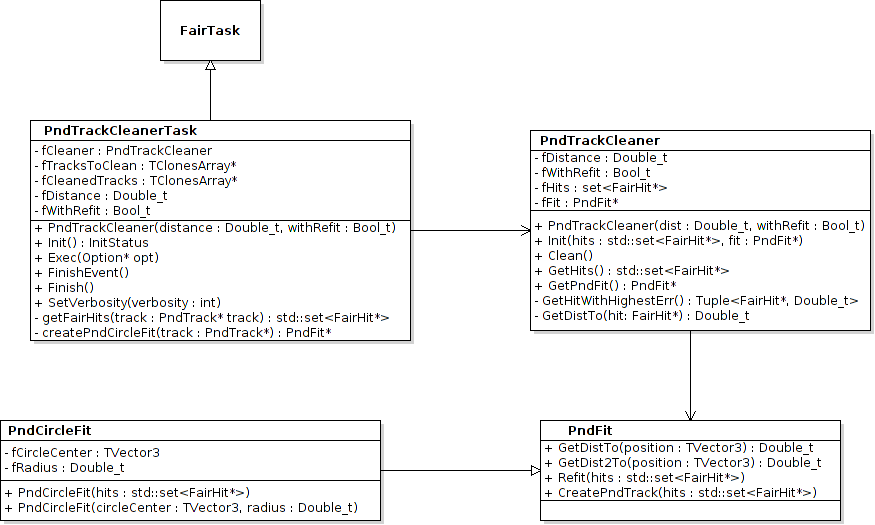
\includegraphics[width=0.9\textwidth]{Bilder/CleanerUML}
	\label{fig:CleanerUML}
	\caption{Veranschaulichung des Entwurfs mittels eines UML-Diagramm}
	
\end{figure}
Der Track-Cleaner wurde nach objektorientierten Grundsätzen entworfen. In Abbildung \ref{fig:CleanerUML} ist ein UML-Diagramm dargestellt, welches den Entwurf verdeutlicht. Es wurde eine Klasse \code{PndTrackCleanerTask} entwickelt, welche den oben erläuterten Vorgaben für eine FairTask genügt. Diese Klasse regelt den Dateizugriff und stellt das Bindeglied zwischen PandaRoot und dem eigentlichen Track-Cleaner dar. Die Klasse \code{PndFit} dient als abstrakte Schnittstelle für eine approximierte Teilchenflugbahn. Diese Schnittstelle umfasst im Wesentlichen die drei Methoden \code{GetDistTo)}, \code{Refit} und \code{CreatePndTrack}. Der Track-Cleaner hält einen Zeiger auf ein Objekt der Klasse PndFit und greift über diese Schnittstelle auf die zum Reinigen der Tracks benötigten Methoden zu. Im konkreten Fall von STT-Hits wird dazu die Unterklasse \code{PndCircleFit} benutzt. Diese legt einen Kreisfit als Approximation zu Grunde und benutzt einen Riemann-Fit um die Kreisparameter zu erzeugen. Der \code{PndTrackCleaner} arbeitet jedoch stets auf der Schnittstelle PndFit, sodass der konkrete Fitting-Algorithmus problemlos ausgetauscht werden kann. Damit es möglich ist, den verwendete Grenzwert \code{fDistance} über ein Skript zu variieren, kann dieser dem PndTrackCleanerTask im Konstruktor übergeben werden. Der Task kann somit den TrackCleaner mit dem übergebenen Wert initialisieren. Dies macht es möglich das ebenfalls parametrisierbare Rekonstruktions-Macro automatisiert mit verschiedenen Grenzwerten aufzurufen. Außerdem wurde ein weiteres Macro implementiert, welches alle Hit von gedrehten Straw-Tubes im Vorfeld aussortiert und einen neuen Root-Branch mit den Namen TracksToClean anlegt. Dieser Branch soll dem TrackCleaner als Eingabe dienen.

\section{Implementation des Verfahrens}
Da der Projektentwurf nun thematisiert wurde, folgen nun Erläuterungen zu den wichtigsten implementierten Methoden.

\subsection{PndTrackCleanerTask}
\begin{description}
	\item[InitStatus Init()] Diese Methode initialisiert zunächst den PndTrackCleaner mit dem Grenzwert fDistance und gibt an ob nach jedem herausgefilterten Punkt ein Refit durchgeführt werden soll. Im Anschluss daran wird der FairRootManager fIoman initialisiert. Dabei handelt es sich um ein Singelton, welches verwendet werden kann, um auf Root-Dateien zugreifen zu können. Danach wird der FairRootManager verwendet um die beiden \code{TClonesArray*} fCleanedTracks und fTracksToClean zu initialisieren. Diese beiden Objekte stellen den Zugriff auf die gleichnamigen Root-Branches her. TracksToClean wird dabei von einem Trackfinder erzeugt und beinhaltet die rekonstruierten Tracks. Der Branch CleanedTracks wird in der Init-Methode neu erstellt und wird mit den bereinigten Tracks gefüllt.
	
	\item[void Exec(Option\_t* opt)] Diese Methode extrahiert die benötigten Tracks aus einem Event und wandelt diese in ein Objekt der Klasse PndFit um. Außerdem werden die zum Cleanen benötigten FairHits von dem Track abgefragt. Mit diesen Daten wird daraufhin der eigentliche Cleaner initialisiert und gestartet. Im Anschluss daran werden die bereinigten Tracks in den neuen Branch CleanedTracks der Root-Datei geschrieben.
	
	\item[void FinishEvent()] Zu Beginn jedes Events werden die Objekte der Klasse TClonesArray* automatisch mit den Daten aus der Root-Datei befüllt. Damit diese beim nächsten Event keine ungültigen Daten mehr enthalten, werden sie in dieser Methode geleert.
	
	\item[void SetVerbosity(int verbosity)] Über diese Methode kann angegeben werden, welche Logging-Informationen bei der Ausführung des TrackCleaners ausgegeben werden sollen. Dabei werden die folgenden Klassifizierungen verwendet:
	\begin{enumerate}
		\item[verbosity=0] Keine Ausgabe
		\item[verbosity=1] Nur Fehler (Default)
		\item[verbosity=2] Fehler und wichtige Logging-Informationen
		\item[verbosity=3] Detailierte Ausgabe, sodass die Programmfunktionalität genau nachvollzogen werden kann.
	\end{enumerate}
	
	\item[std::set<FairHit*> getFairHits(PndTrack* track)] Diese Methode extrahiert aus dem übergebenen PndTrack die Menge an FairHits, welche dem Track zugeordnet worden ist.
	
	\item[PndFit* createPndCircleFit(PndTrack* track)] Um den TrackCleaner zu initialisieren, wird ein Objekt der Klasse PndFit benötigt. In dieser Methode wird dazu ein Objekt der Klasse PndCircleFit erstellt, welches die Teilchenflugbahn des übergebenen Tracks approximiert.
\end{description}

\subsection{PndTrackCleaner}
\begin{description}
	\item[void Clean()] Diese Methode führt die eigentliche Bereinigung des Tracks durch. Dazu wird in einer Schleife die private Methode GetHitWithHighestErr aufgerufen und überprüft, ob der minimale Abstand des zurückgegebenen Hits vom approximierten Track größer ist als zugelassene Grenzwert. Ist dies der Fall wird der gefundene Hit entfernt, evtl. ein Refit ausgeführt und das Verfahren dann wiederholt. Falls der Grenzwert nicht überschritten wird, kann das Verfahren hier abgebrochen werden.
	
	\item[Tuple<FairHit*, Double\_t> GetHitWithHighestErr()] In dieser Methode wird für jeden Hit der minimalen Abstand zum approximierten Track berechnet und der Hit ausgewählt, bei dem dieser Abstand am größten ist. Danach wird ein Tupel zurückgegeben, welches den ausgewählten Hit und den Abstand zum Track enthält.
	
	\item[Double\_t GetDistTo(FairHit* hit)] Diese Methode bestimmt den Abstand eines FairHits vom aktuellen Fit. Dazu wird auf die Methide PndFit::GetDist2To zurückgegriffen.
	
	\item[std::set<FairHit*> GetHits()] Nachdem das Reinigen eines Tracks abgeschlossen ist, wird der bereinigte Track vom PndTrackCleanerTask wieder in die Root-Datei geschrieben. Da dazu die verbleibenden Hits benötigt werden, können diese über die Methode GetHits abgefragt werden.
\end{description}

\subsection{PndCircleFit}
\begin{description}
	\item[Double\_t getDistTo(TVector3 position)] In dieser Methode wird zunächst der Abstandsvektor des übergebenen Punktes vom Kreismittelpunkt berechnet. Im Anschluss daran wird von der Norm dieses Vektors der Kreisradius subtrahiert um somit den Abstand des Punktes von der Kreisbahn zu berechnen. Da es sich beim Kreisfit um eine Projektion in die Ebene handelt, wird vor der Berechnung die z-Komponente des übergebenen Vektors auf 0 gesetzt.


	\item[void Refit(std::set<FairHit*> hits)] Nachdem ein Hit aus dem aktuellen Track entfernt wurde, muss gegebenenfalls ein Refit ausgeführt werden. Dazu wird in dieser Methode die Klasse PndRiemannFit benutzt um die Kreisparameter ausgehend von den übergebenen Hits anzupassen.

	\item[PndTrack CreatePndTrack(std::set<FairHit*> hits)] In dieser Methode wird ausgehend von den übergebenen Hits ein PndTrack erstellt, sodass dieser in der Root-Datei gespeichert werden kann. Dazu wird die Methode getPndTrack der Klasse PndRiemannTrack verwendet.
\end{description}
\chapter{Analyse}
Abschließend soll nun die Funktionalität des TrackCleaners untersucht und bewertet werden. Dazu wird zunächst die Funktionsweise des Cleaners an einem exemplarischen Fall demonstriert. Im Anschluss daran wird das Laufzeitverhalten und die Qualität des Bereinigens analysiert und bewertet. Des Weiteren wird dokumentiert, wie die optimale Distanz, ab welcher ein Hit aussortiert wird, bestimmt wurde.

\section{Analyse der Funktionalität}
Root bietet die Möglichkeit die simulierten Events zu visualisieren. Dazu kommt das Tool Eve zum Einsatz, welches in der Lage ist eine Root-Datei auszulesen und Tracks, Mote-Carlo-Points und Hits graphisch darzustellen. Abbildung \ref{fig:points} zeigt ein Event mit zwei physikalischen Tracks, welche von zwei verschiedenen Teilchen verursacht wurden. Das erste Teilchen(grün) bewegte sich vom Stoßpunkt aus auf einer vergleichsweise geradlinigen Flugbahn aus dem STT heraus. Das zweite Teilchen(weiß) bewegt sich auf einer Kreisbahn mehrere Male durch den STT und kreuzt dabei auch die Flugbahn des ersten Teilchens. Die magentafarbenen Punkte stellen die Ponte-Carlo-Points dar. An diesen Stellen haben die beiden Teilchen also die Straw-Tubes durchflogen. Betrachtet wird nun die Rekonstruktion des grünen Tracks. 

\begin{figure}
  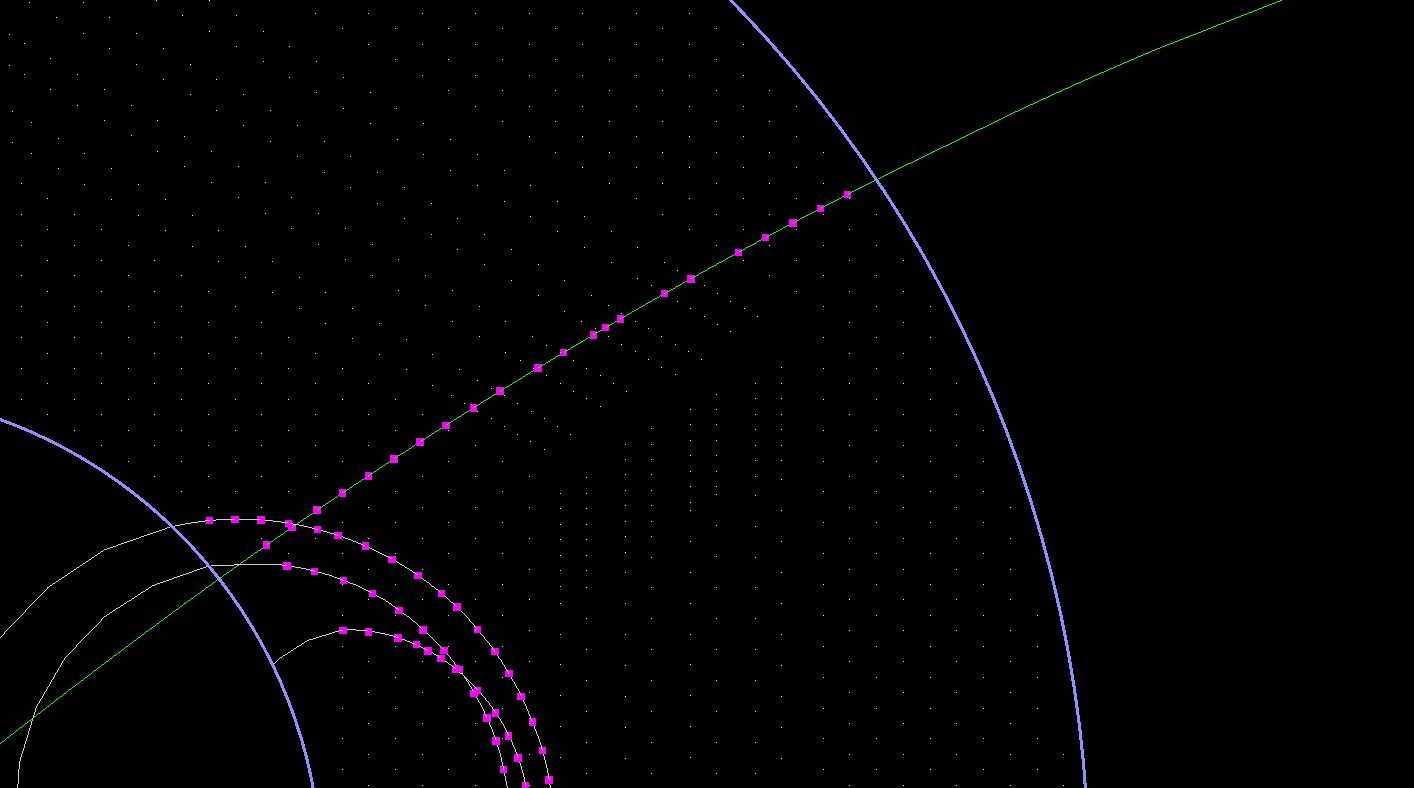
\includegraphics[width=0.9\textwidth]{Bilder/Points2}
	\label{fig:points}
	\caption{Visualisierung eines Events mit zwei Tracks}
\end{figure}

In Abbildung \ref{fig:hits} sind die Hits dargestellt, welche von einem Track-Cleaner diesem Track zugeordnet wurden. In Rot wurde die approximierte Kreisbahn dargestellt. Zunächst fällt auf, dass die Hits im Gegensatz zu den Points nicht direkt auf der Kreisbahn liegen, da sie am Mittelpunkt der getroffenen Straw-Tube dargestellt werden. Folglich besitzen auch die korrekt rekonstruierten Hits meist einen gewissen Abstand vom Track. Außerdem sind die gedrehten Straw-Tubes aus den oben genannten Gründen vom Track entfernt worden. Des Weiteren ist zu bemerken, dass sich am inneren Rand des STTs vier Hits mit einem vergleichsweise großen Abstand zum Track befinden. Beim Vergleich beider Abbildungen lässt sich feststellen, dass sich diesen Punkten keinen Points zuordnen lassen, welche zum grünen Track gehören. In der unmittelbaren Umgebung existieren jedoch einige Points, welche dem weißen Track zuzuordnen sind. Folglich sind diese vier Hits fehlerhaft zugeordnet worden.

\begin{figure}
  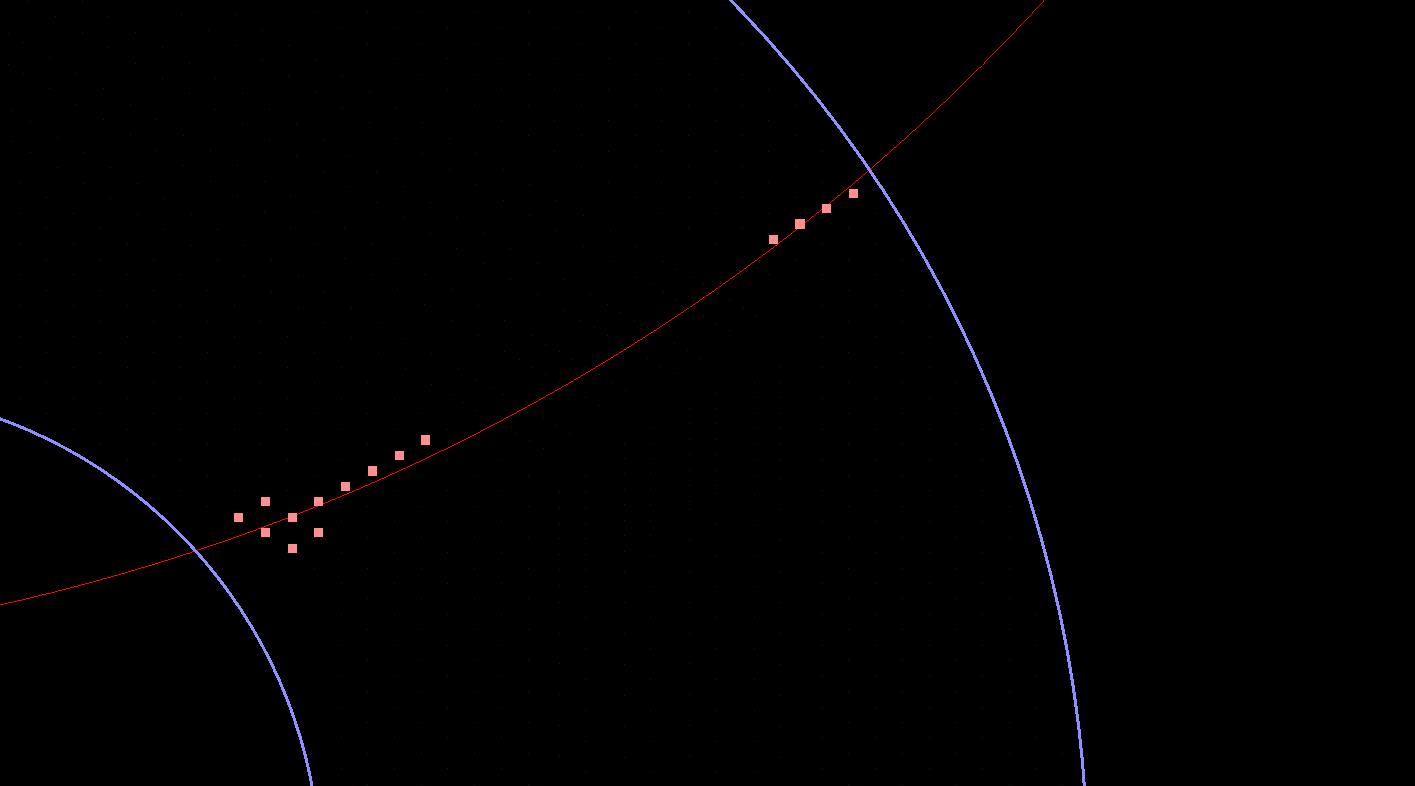
\includegraphics[width=0.9\textwidth]{Bilder/HitsApprox}
	\label{fig:hits}
	\caption{Visualisierung des rekonstruierten Tracks mit den zugeordneten STT-Hits}
\end{figure}

Der vorliegende, rekonstruierte Track wird nun vom TrackCleaner bereinigt. Das Ergebnis ist in Abbildung \ref{fig:cleaned} zu sehen. Es ist zu sehen, dass die beiden unteren fehlerhaften Hits aussortiert worden sind und eine verbesserte Approximation erstellt wurde. Die oberen beiden Fehlerhaften Hits wurden nicht entfernt. Dies hängt damit zusammen, dass im vorliegenden Beispiel die Distanz 0.6 benutzt wurde und die oberen Hits diesen Grenzwert nicht überschreiten.

\begin{figure}
  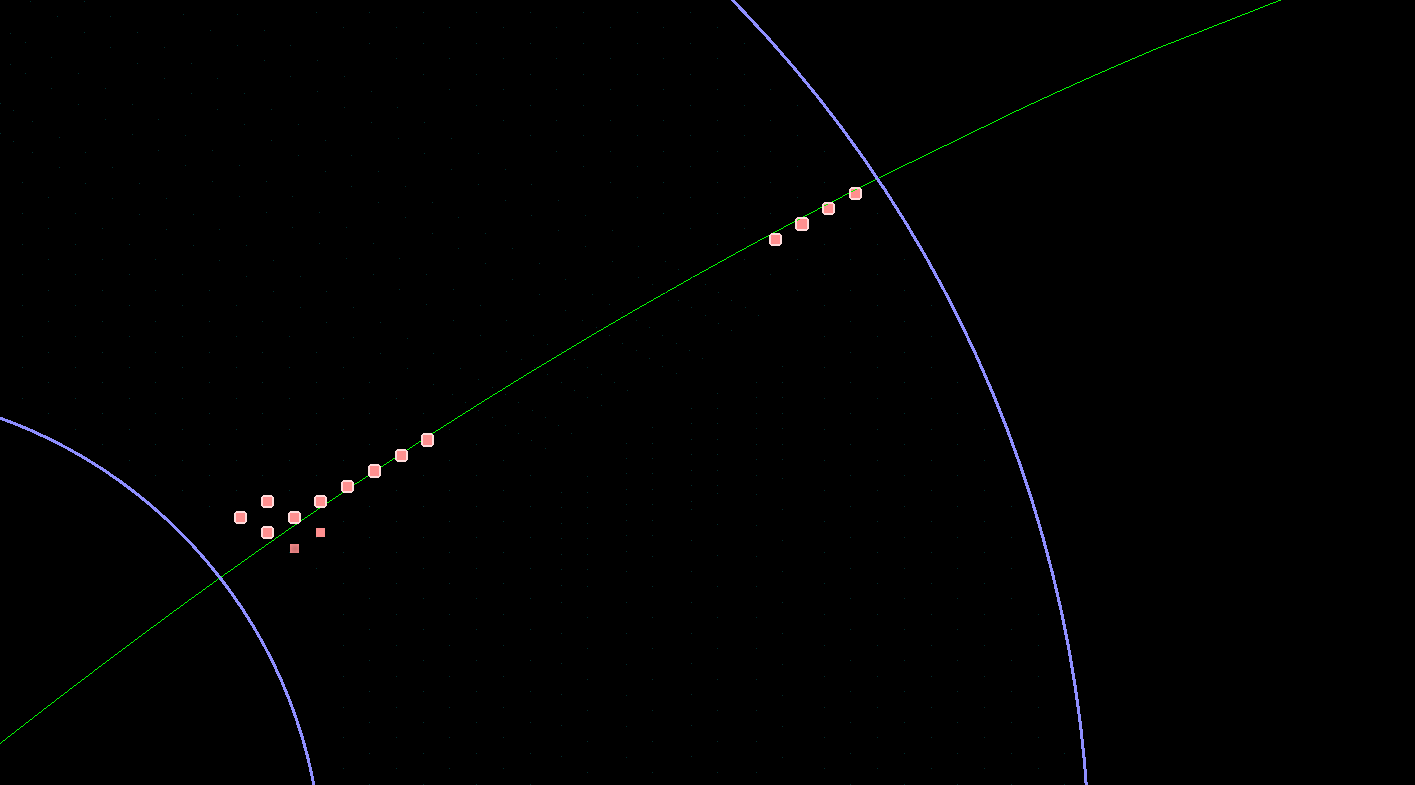
\includegraphics[width=0.9\textwidth]{Bilder/CleanedWithTrack}
	\label{fig:cleaned}
	\caption{Visualisierung des bereinigten Tracks}
\end{figure}

\section{Qualitätsanalyse}
Zur genauen Analyse des Algorithmus wurde eine Analysetask entwickelt. Diese lädt zunächst die Root-Branches CleanedTracks und TracksToClean. Da bei einer Simulation die Daten der physikalischen Tracks vorliegen, ist es nun möglich, zu jedem Hit der beiden Tracks die ID des zugehörigen MC-Tracks zu bestimmen. Im Anschluss daran wird der MC-Track bestimmt, welcher die meisten zugehörigen Hits im zu bereinigten Track enthält. Es wird dann angenommen, dass dieser Track rekonstruiert werden sollte. Alle Hits mit einer identischen Track-ID sind folglich korrekt zugeordnet und alle Hits mit einer anderen Track-ID sind fehlerhaft. Danach werden über die folgende Mengenoperation die Hits bestimmt, welche vom Cleaner aussortiert wurden.

\begin{Definition}
Sei A die Menge der Hits, welche zu einem bereinigten Track gehören und B die Menge der Hits, welche zu dem entsprechenden, noch nicht bereinigten Track gehören. Dann enthält C=B\textbackslash A genau die Hits, welche vom TrackCleaner aussortiert wurden.
\end{Definition}

Abschließend wird dann zu jeden Hit $ h \in C $ die TrackID bestimmt, und somit beurteilt, ob es sich um einen korrekt aussortierten Hit handelt. Das Ergebnis der Analyse wird dann zusammen mit der beim Bereinigen benutzten Distanz an eine CSV-Datei angehängt, um die Ergebnisse später automatisiert weiterverarbeiten zu können.

\section{Laufzeitverhalten}
Bei der Analyse des Laufzeitverhaltens ergaben sich die in \ref{tab: resultsRuntime} dargestellten Ergebnisse. Die Methoden Init und Exec beziehen sich auf die Klasse PndTrackCleanerTask, die Methode Clean bezieht sich auf den PndTrackCleaner.

\begin{figure}
\begin{center}
\begin{tabular}{ |c|c|}
	\hline
	Methode & Laufzeit\\
	\hline
	Init & $6 \cdot 10^{-5} s$ \\
	Exec & $2.027 \cdot 10^{-6} s$\\
	Clean & $7 \cdot 10^{-9} s$\\
	\hline
\end{tabular}
\end{center}
\caption{Ergebnisse der Laufzeitanalyse}
\label{tab: resultsRuntime}
\end{figure}

\section{Bestimmung der optimalen Distanz}
Es soll nun im Rahmen einer Parameterstudie die optimale Distanz bestimmt werden. Dazu wurde ein Skript entwickelt, welches sowohl die Rekonstruktion als auch die Analyse mit unterschiedlichen Distanzen startet. Die CSV Datei wird dann mit den Ergebnissen der Analyse gefüllt. Dabei ergaben sich die in Tabelle \ref{tab: results} dargestellten Ergebnisse. Die hier dargestellte Simulation beinhaltete 1000 Events mit insgesamt 48152 STT-Hits von ausschließlich nicht gedrehten Straw-Tubes. Der erste Eintrag der Tabelle stellt die Ergebnisse dar, welche bei einer Distanz von null erzielt werden. Da hierbei ausnahmslos alle Hits aussortiert werden, macht diese Distanz wenig Sinn, liefert jedoch Informationen über die Beschaffenheit der vorliegenden Stichprobe. Da 1889 Hits korrekt entfernt wurden, hat in diesen Fällen der Trackfinding-Algorithmus einen Fehler gemacht. Die Entfernung der übrigen 46263 Hits war hingegen inkorrekt, folglich wurden diese Hits korrekt zugeordnet.

\begin{figure}
\begin{center}
\begin{tabular}{ |c|c|c|c|}
	\hline
	Distanz & aussortierte Hits & davon korrekt entfernt & davon fehlerhaft entfernt\\
	\hline
0	&   48152 &1889 & 46263\\
0.1	&	12824 & 989	& 11835\\
0.2	&	5144	  & 831	& 4313\\
0.3	&	2153	  & 661	& 1492\\
0.4	&	1034  &	455	& 579\\
0.5	&	685	  & 345	& 340\\
0.6	&	477	  & 249	& 228\\
0.7	&	340	  & 178	& 162\\
0.8	&	239   & 	120	& 119\\
0.9	&	162	  & 71	& 91\\
1	&	126   & 	53	& 73\\
	\hline
\end{tabular}
\end{center}
\caption{Ergebnisse der Analysetask}
\label{tab: results}
\end{figure}

In Abbildung \ref{fig:results} finden sich diese Ergebnisse in Form eines Balkendiagramms wieder. Aus Tabelle und Graphik geht hervor, dass bei Distanzen welche kleiner sind als 0.3, die fehlerhaft entfernten Hits deutlich überwiegen. Die Anzahl der fehlerhaften Hits fällt jedoch bei größeren Distanzen recht schnell ab. Insgesamt scheint hier ein Zusammenhang vorzuliegen, welcher sich asymptotisch wie $-e^x$ verhält. Die Anzahl der korrekt entfernten Hits liegt für kleine Distanzen deutlich unter den fehlerhaft entfernten Hits und fällt dann für größere Distanzen ebenfalls ab. Der hier vorliegende Abfall ist jedoch deutlich geringer als bei den fehlerhaft aussortierten Hits. Bei den Distanzen 0.5 - 0.8 überwiegt daher die Anzahl der korrekt aussortierten die Anzahl der fehlerhaft aussortierten Hits. Bei Distanzen überhalb von 0.8 existieren dann wieder mehr fehlerhaft aussortierte Hits. Bei der Betrachtung der betreffenden Tracks ist aufgefallen, dass dies auf schlechte eine Approximation des physikalischen Tracks zurückzuführen ist. Abbildung \ref{fig:Problem} verdeutlicht die Problematik. Die drei markierten Hits wurden fehlerhaft zum Track hinzugefügt und beeinflussen somit die Approximation. Dies hat zur Folge, dass Hits aus dem korrekten Track einen größeren Abstand zum Kreisfit haben und somit entfernt werden. Es wurde beobachtet, dass bei fehlerfrei rekonstruierten Tracks nur sehr selten Hits fehlerhaft entfernt wurden.

\begin{figure}
\begin{center}
  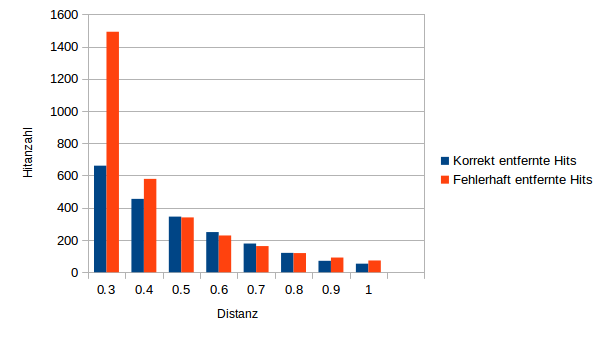
\includegraphics[width=0.9\textwidth]{Bilder/Results}
	\label{fig:results}
	\caption{Visualisierte Ergebnisse der Analysetask}
\end{center}
\end{figure}

\begin{figure}
\begin{center}
  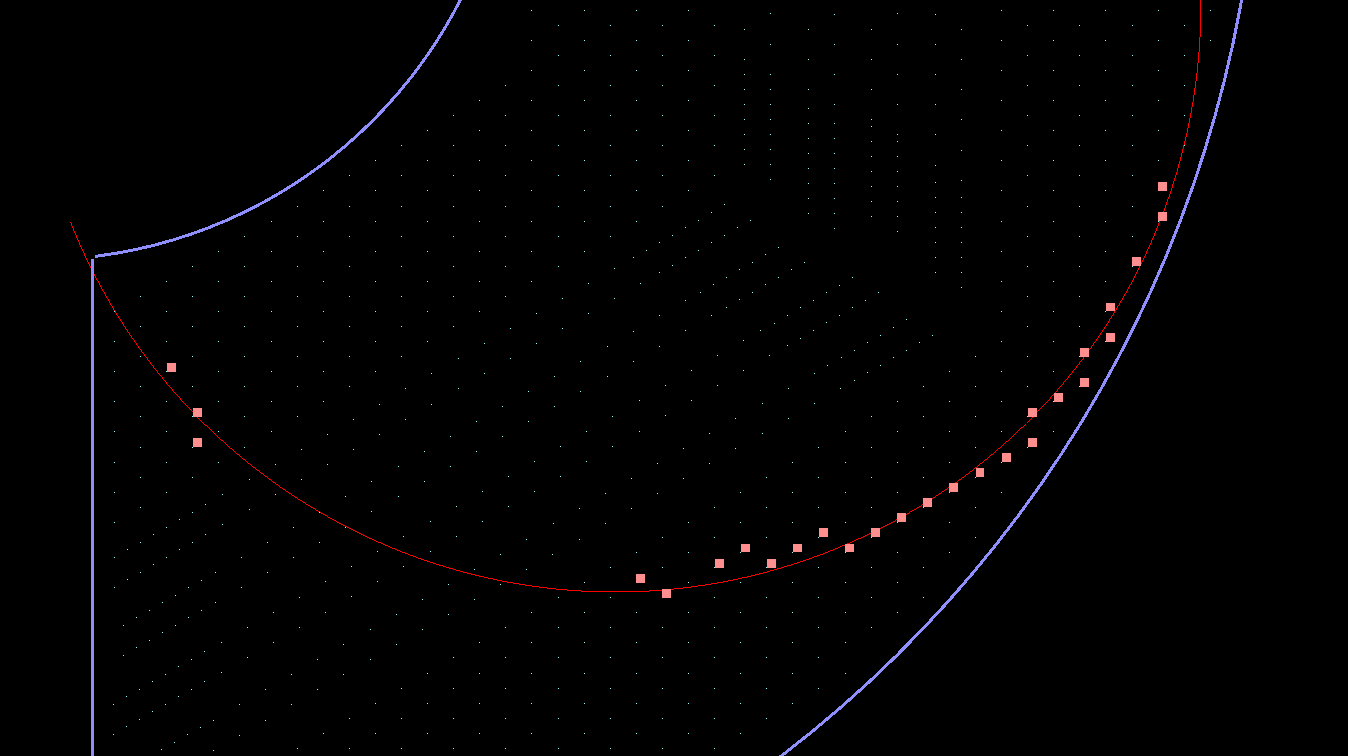
\includegraphics[width=0.9\textwidth]{Bilder/Problems}
	\label{fig:Problem}
	\caption{Visualisierung eines Events, welches beim bereinigen Probleme bereitet}
\end{center}
\end{figure}
\chapter{Fazit und Ausblick}
Die durchgeführte Analyse lieferte Informationen über die Qualität des implementierten TrackCleaners. Wird als Gütekriterium die Differenz der fehlerhaft entfernten Hits und der korrekt entfernten Hits zu Grunde gelegt ergibt sich eine optimale Distanz von 0.6, da hier die Anzahl der korrekt aussortierten Hits die Anzahl der fehlerhaft aussortierten Hits um 21 übersteigt.
Eine Differenz von 21 stellt bei 1000 Simulierten Events jedoch keine signifikante Überzahl der korrekt entfernten Hits dar. Selbst bei optimaler Distanz liegt die Anzahl der korrekt entfernten Hits nur minimal über der Anzahl der fehlerhaft entfernten Hits. Dabei kommt noch erschwerend hinzu, dass im Zweifelsfall wünschenswerter ist einen Track mit falschen Hits zu rekonstruieren als korrekte Hits aus einem Track zu entfernen. Die hohe Anzahl fehlerhaft entfernter Hits ist darauf zurückzuführen, dass sich bei rekonstruierten Tracks mit einigen fehlerhaften Hits schlechte Approximation ergeben. Da die Approximation meist besonders schlecht ist, wenn die fehlerhaften Hits weit von den übrigen Hits entfernt liegen könnten in einer weiterführenden Arbeit diese Tracks erkannt und vom Bereinigen ausgeschlossen werden. Das Laufzeitverhalten des TrackCleaners ist hingegen positiver zu beurteilen. Das bereinigen der Tracks nach einer Rekonstruktion würde das Laufzeitverhalten nicht signifikant beeinflussen und ist somit für den Einsatz in einem Online-Tracker geeignet. Darüber hinaus wäre der TrackCleaner sehr einfach zu parallelisieren, da die Bereinigung eines Tracks völlig unabhängig von der Verarbeitung der übrigen Tracks funktioniert. Zusammenfassend lässt sich sagen, dass sich der TrackCleaner  ohne weitgehende Verbesserungen nur bedingt zum Bereinigen von Tracks einsetzen lässt, da die Anzahl der fehlerhaft entfernten Hits zu hoch ist.
 
\bibliographystyle{plain} 
\bibliography{Literatur}

 
\end{document}